\section{Two families of regions and the area bound}
\label{sec:geometry}

The amplified collar estimate controls the mutual information between one
region and any collection of sites outside its collar.  To use it in an
entropy chain, we need to divide $A$ into two families: within each family,
the collar of a region must avoid all regions that precede it.  We group
cells in distance layers into primary tiles separated by sparse strips.
Filling the strips with suitable labels leaves only point contacts between
regions of the same family.  We separate those contacts by recursively
replacing small squares around them.  The sites left at the end of this
construction, and all the mutual-information errors, will be bounded by
the number of cut edges.

The construction takes place in the ambient plane.  Its use of ambient
distance only supplies sufficient conditions for separation in the induced
graph: every graph path of length $r$ has ambient displacement at most $r$.
We never require an ambiently short path to exist in the domain.

\subsection{The entropy cancellation}

We first isolate the elementary reason that two families suffice.  This
also specifies precisely the separation property that the geometry must
provide.

\begin{lemma}[Two-family entropy cancellation]
\label{geometry:cancellation}
Let $\psi$ be a pure state on a finite tensor product with site set
$\Lambda$.  Suppose that
\[
 A=D\mathbin{\dot\cup}\bigcup_{i\in\mathcal I_0}X_i
       \mathbin{\dot\cup}\bigcup_{i\in\mathcal I_1}X_i
 \subseteq\Lambda
\]
is a partition into disjoint sets, and fix an order on each finite index
set $\mathcal I_f$, $f\in\{0,1\}$.  Write $B=\Lambda\setminus A$.
If
\[
 I_\psi\left(X_i:B\cup
       \bigcup_{\substack{j\in\mathcal I_f\\j<i}}X_j\right)
 \le \varepsilon_i
 \qquad(i\in\mathcal I_f),
\]
then
\[
 S_\psi(A)\le S_\psi(D)+\frac12\sum_i\varepsilon_i.
\]
\end{lemma}

\begin{proof}
Write $A_f=\bigcup_{i\in\mathcal I_f}X_i$ and
$E_f=\sum_{i\in\mathcal I_f}\varepsilon_i$.  The entropy chain rule and
purity give
\[
 S_\psi(BA_f)
 \ge S_\psi(B)+\sum_{i\in\mathcal I_f}S_\psi(X_i)-E_f
 =S_\psi(A)+\sum_{i\in\mathcal I_f}S_\psi(X_i)-E_f.
\]
On the other hand, purity and subadditivity give
\[
 S_\psi(BA_f)=S_\psi(DA_{1-f})
 \le S_\psi(D)+\sum_{i\in\mathcal I_{1-f}}S_\psi(X_i).
\]
Adding the inequalities for $f=0$ and $f=1$ cancels every individual tile
entropy and proves the claim.
\end{proof}

\subsection{The geometric statement}

Keep the exponent $\beta=1-2\cdot10^{-6}$ from
Proposition~\ref{prop:amplification}, and put
\begin{equation}
\label{geometry:exponents}
 \delta_0=2\cdot10^{-7},\qquad
 \zeta=1-\frac{\delta_0}{2},\qquad
 \rho_0=\frac{1+\beta}{2},\qquad
 \ell=10^{-5}.
\end{equation}
The inequalities we shall use are
\begin{equation}
\label{geometry:exponent-gaps}
 (1+2\delta_0)\beta<\zeta<1,\qquad
 (1+2\delta_0)(1-\ell)<1,\qquad
 1-\ell<\beta<\rho_0<1.
\end{equation}
All their gaps are fixed positive numbers.  Thresholds depending on these
gaps may therefore be chosen independently of $\Lambda$ and $A$.

A \emph{birth region} below is the bounded closed planar region assigned
to a tile when that tile is created.  Later steps only delete points from
that tile.  Its \emph{actual region} is the interior of its birth region remaining
after all deletions.  Different pieces with the same tile identifier are treated as
one region; neither a birth region nor an actual region is required to be
connected.  Its ambient lattice template is the intersection of its birth
region with $\Z^2$.  We distinguish the two family labels $0,1$ from the
two sides $A,\Lambda\setminus A$ of the physical cut.

\begin{proposition}[Two families with separated birth templates]
\label{prop:two-families}
Fix the constants $D_0$ and $C_{\mathrm{tpl}}$ in
Definition~\ref{scanner:template}, and a lower scale threshold $n_*\ge1$.
There is a constant $C$ with the following property.  Let $\Lambda$ be a
finite induced subgraph of the square lattice, let $A\subseteq\Lambda$,
and suppose that $b=|\partial_\Lambda A|>0$.  Let $Z$ be the set of
endpoints of those cut edges.

There are a set $D\subseteq A$, a finite ordered collection of disjoint
nonempty sets $X_i\subseteq A$, labels $f_i\in\{0,1\}$, ambient templates
$T_i\subset\Z^2$, and integers $n_i\ge n_*$ such that:
\begin{enumerate}
\item
$A=D\mathbin{\dot\cup}\bigcup_iX_i$ and $|D|\le Cb$.
\item
$X_i\subseteq A\cap T_i$.  Each $T_i$ is a template of
Definition~\ref{scanner:template}: it is a union of $N_i$ lattice samples
of closed convex rectangles or triangles with side slopes
$0,\infty,1,-1$, each of sup-norm diameter at most $s_i$, where
\[
 \diam_\infty T_i\le n_i,\qquad
 n_i\ge C_{\mathrm{tpl}}N_i(s_i+1),\qquad
 \dist_\infty(T_i,Z)>4D_0s_i.
\]
Moreover $L_i=\lfloor n_i^{1-\ell}\rfloor\le s_i$.
\item
The templates satisfy
\begin{align}
 \dist_\infty(T_i,Z)&>2n_i^\beta,\label{geometry:cut-clearance}\\
 \dist_\infty\left(T_i,
       \bigcup_{\substack{j<i\\f_j=f_i}}X_j\right)
       &>2n_i^\beta.\label{geometry:ordered-clearance}
\end{align}
As usual, the distance to the empty set is infinite.
\item
The scale losses are summable:
\[
 \sum_i n_i^{-100}\le Cb.
\]
\end{enumerate}
The constant $C$ may depend on the fixed template constants and on $n_*$,
but not on the domain or cut.
\end{proposition}

We prove the proposition in stages.  First we construct layers with
sparse connecting strips.  Next we remove their same-family vertex
contacts.  Finally we verify separation for the entire birth templates,
not merely for the smaller actual regions.

\subsection{Layers and sparse strips}

Fix a translated origin
\[
 o=(\sqrt2,\sqrt3).
\]
Each of $o_1,o_2,o_1+o_2,o_1-o_2$ is nonintegral.  On every dyadic scale
$r=2^k$, use the half-open cells
\[
 C_{k,z}=o+r\bigl(z+[0,1)^2\bigr),\qquad z\in\Z^2.
\]
These grids are nested.  Half-open cells determine indices; their closures
will determine birth regions.  Choose an integer $C_0$ sufficiently large
compared with $D_0$, for example $C_0>100(D_0+1)$, and define
\[
 \mathcal Z_k=\{z:C_{k,z}\cap Z\ne\varnothing\},\qquad
 N_k=\bigcup_{\dist_\infty(z,\mathcal Z_k)\le C_0}C_{k,z}.
\]
Here the distance in the subscript is the sup distance between integer
cell indices.  Passing to parents shows that $N_k\subseteq N_{k+1}$:
if two child indices differ by at most $C_0$ in each coordinate, their
parent indices also differ by at most $C_0$.  The sets $N_k$ exhaust the
plane, since $Z\ne\varnothing$ and $C_0\ge2$.

For a lower index $k_0$ to be fixed later, regard $N_{k_0}$ as one
\emph{dummy tile}, labeled by the parity of $k_0-1$.  Its points will
initially be exceptional.  For $k\ge k_0$, the layer
\[
 D_k=N_{k+1}\setminus N_k
\]
is a union of cells of side $r=2^k$.  There are at most $C|Z|\le Cb$ of
these cells: $N_{k+1}$ has at most $(2C_0+1)^2|Z|$ cells of side $2r$,
each of which has four children.  The cell-index definition also gives
\begin{equation}
\label{geometry:layer-distance}
 C_0r\le\dist_\infty(x,Z)\le2(C_0+1)r
 \qquad(x\in\overline{D_k}).
\end{equation}
For the lower bound, a cell outside $N_k$ differs from every
endpoint-occupied cell by at least $C_0+1$ in one coordinate.  For the
upper bound use its parent in $N_{k+1}$.

The function $x\mapsto\dist_\infty(x,Z)$ is 1-Lipschitz.  Consequently,
if $h\ge k+2$, then
\begin{equation}
\label{geometry:nonadjacent}
 \dist_\infty(\overline{D_k},\overline{D_h})
 \ge C_0 2^h-2(C_0+1)2^k
 \ge \frac{C_0-1}{2}\,2^h.
\end{equation}
Thus only the same layer or a neighboring layer can occur near a region
whose size is much smaller than its layer scale.

In $D_k$ put
\[
 s_k=2^{\lfloor(1+\delta_0)k\rfloor},\qquad
 t_k=2^{\lfloor\zeta k\rfloor}.
\]
For sufficiently large $k_0$, we have $t_k\mid r\mid s_k$ and
$t_k\ll r\ll s_k$, uniformly as $k\to\infty$.  Here $r$ is the
layer-cell scale, $s_k$ is the pitch used to group fragments into primary
tiles, and $t_k$ will be the width of the strips separating those tiles.
The larger pitch makes the strips sparse within a layer; the $r$-cells
will later supply the small pieces in each primary's template.
The fine cells of side $t_k$ have origin $o$.  Choose two residue classes
modulo $s_k/t_k$, one for each coordinate.  A fine cell is called a \emph{belt cell} if either
of its two indices lies in the corresponding selected residue class.
The remaining fine cells lie in open pitch interiors, each a square
between successive belt strips.  For each such pitch interior, give all
its fragments in $D_k$ one primary-tile identifier and the label
$k\bmod2$.

The shifts can be chosen so that few belt cells meet the layer.  Indeed,
the layer contains at most $Cb(r/t_k)^2$ fine cells before any shift is
chosen.  Under a uniform choice of the two residue classes, each is a
belt cell with probability at most $2t_k/s_k$.  Hence some shift satisfies
\begin{equation}
\label{geometry:belt-count}
 \#\{\text{belt cells in }D_k\}
 \le Cb\frac{r^2}{s_kt_k}
 \le Cb\,2^{-k\delta_0/2}.
\end{equation}
We fix such a shift in each layer.  This is an averaging argument on a
predetermined collection of cells; no property of the state enters it.
The geometric decay in $k$ absorbs any fixed power of $k$.  Below,
\eqref{geometry:descendant-count} will bound the number of repairs
descended from one contact by just such a power, so sparse strips also
control the total number of tiles created by the repairs.

Each $r$-cell meets only a bounded number of pitch interiors, so there
are at most $Cb$ primary tiles in a layer.  The birth region of one
primary is a union of at most
\begin{equation}
\label{geometry:primary-pieces}
 C(s_k/r+2)^2
\end{equation}
closed rectangles of sup-norm diameter at most $r$, obtained as closures
of the intersections of that pitch interior with the $r$-cells of the
layer.  Its whole sup-norm diameter is at most $s_k$.  Distinct primaries in the same layer are separated by a belt
strip of width at least $t_k$.  Primaries in adjacent layers have opposite
labels; primaries of the same label in different layers satisfy
\eqref{geometry:nonadjacent}.
Figure~\ref{geometry:layer-picture} shows why a primary can have several
components even though it occupies a single pitch interior.

\begin{figure}[H]
\centering
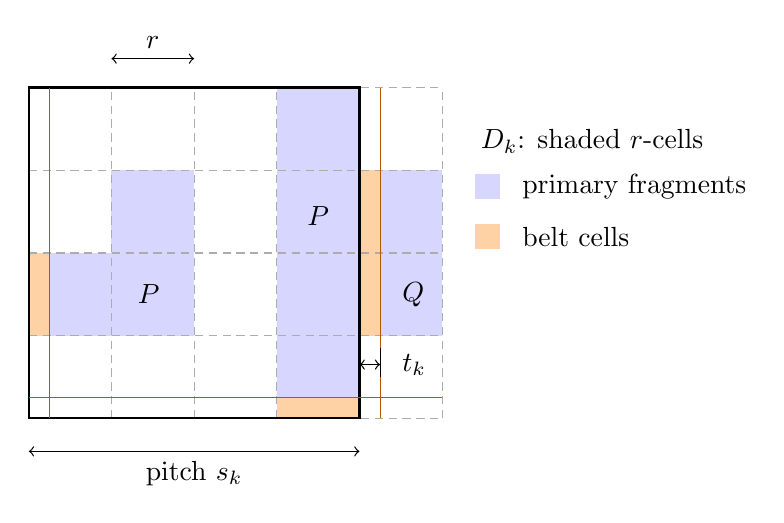
\begin{tikzpicture}[scale=1.05, line width=.45pt]
 \foreach \x/\y in {0/1,1/1,1/2,3/0,3/1,3/2,3/3,4/1,4/2}
   {\fill[blue!16] (\x,\y) rectangle +(1,1);}
 \fill[orange!35] (0,1) rectangle (.25,2);
 \fill[orange!35] (3,0) rectangle (4,.25);
 \fill[orange!35] (4,1) rectangle (4.25,3);
 \draw[step=1,gray!65,densely dashed] (0,0) grid (5,4);
 \draw[thick] (0,0) rectangle (4,4);
 \draw[orange!70!black] (.25,0)--(.25,4)
                          (4.25,0)--(4.25,4)
                          (0,.25)--(5,.25);
 \node at (1.45,1.5) {$P$};
 \node at (3.5,2.45) {$P$};
 \node at (4.65,1.5) {$Q$};
 \node[anchor=west] at (5.35,3.35) {$D_k$: shaded $r$-cells};
 \fill[blue!16] (5.4,2.65) rectangle (5.7,2.95);
 \node[anchor=west] at (5.85,2.8) {primary fragments};
 \fill[orange!35] (5.4,2.05) rectangle (5.7,2.35);
 \node[anchor=west] at (5.85,2.2) {belt cells};
 \draw[<->] (0,-.4)--(4,-.4);
 \node[below] at (2,-.4) {pitch $s_k$};
 \draw[<->] (1,4.35)--(2,4.35);
 \node[above] at (1.5,4.35) {$r$};
 \draw[<->] (4,.65)--(4.25,.65);
 \draw (4,.5)--(4,.85) (4.25,.5)--(4.25,.85);
 \node[anchor=west] at (4.4,.65) {$t_k$};
\end{tikzpicture}
\caption{A schematic portion of one ambient layer, not to scale.
Dashed lines mark the $r$-cells.  The thick square is one pitch cell;
its interior after removing the belt strips has side $s_k-t_k$.
All blue fragments in that interior share the primary identifier $P$,
even when disconnected.  The neighboring fragment has identifier $Q$.
Both primaries have family label $k\bmod2$; the orange belt cells are
filled and labeled in the next step.  The drawing concerns the ambient
layer $D_k$, before intersection with the physical set $A$.}
\label{geometry:layer-picture}
\end{figure}

\subsection{Filling the belts}

The remaining construction colors the belt cells while making every
positive-length interface between different tile identifiers join
opposite labels.  Point contacts will be dealt with separately.

Adjacent layer fine meshes have side ratio either 1 or 2.  They have a
common translated dyadic origin, including after the pitch shifts, which
were by multiples of their fine-cell sides.  Divide a side of a belt
cell at any corner of an opposing cell.  A larger side can be divided
only at its midpoint.  Along each resulting elementary segment, the
opposing region is either one primary or dummy tile, or one elementary
segment of another belt cell.  A layer boundary cannot change in the
interior of such a segment: layer edges lie on the coarser dyadic grids.

Join the center of each belt cell to the endpoints of its elementary
segments.  This makes a fan of at most eight triangles, with edges of
slopes $0,\infty,1,-1$.  A triangle facing a primary or dummy tile receives
the opposite label.  On a segment shared by two belt cells, assign any
opposite pair of labels to its two incident triangles, consistently on
both sides.  Within each belt cell merge each cyclic run of consecutive
triangles with the same label into one tile identifier.  Distinct runs
remain distinct identifiers; if all labels agree, the whole cell is one
tile.

Every positive-length interface between distinct identifiers now joins
opposite labels.  Across a cell side this follows from the assignment;
inside a fan it follows from merging equal-label neighbors.  Primaries
were already separated in the same layer, and adjacent-layer primaries
have opposite labels.  Thus a same-label contact between distinct tiles
can only be a point, and every such contact involves a belt cell.

Mark the center, the four corners, and the four side midpoints of every
belt cell.  Some midpoint marks are unnecessary for its fan, but adding
them simplifies the recursion.  Deduplicate coincident marks, assigning
a mark $v$ the scale $S_v$ equal to the smallest side length of a belt
cell that marked it.  There are at most nine times as many initial marks
as belt cells.

\begin{lemma}[Isolated stars of the initial mesh]
\label{geometry:initial-stars}
There is an absolute constant $a_0>0$, independent of the layer and the
chosen shifts, such that, on taking $k_0$ sufficiently large:
\begin{enumerate}
\item
Distinct marks $v,w$ satisfy
$\norm{v-w}_\infty\ge a_0\max(S_v,S_w)$.
\item
In the square $v+[-a_0S_v,a_0S_v]^2$, all active boundaries are straight
rays from $v$ in the eight axis and diagonal directions.  Each sector
between consecutive active rays has one tile identifier, and consecutive
sectors have opposite labels.  If there is no active ray, the square is
in one tile.
\end{enumerate}
An active boundary here means an interface of distinct identifiers;
seams removed by a merge are not boundaries.
\end{lemma}

\begin{proof}
Consider a belt cell of side $t=t_k$.  In its $10t$-neighborhood only its
own and adjacent layers can occur, by \eqref{geometry:nonadjacent} and
$t_k/2^k\to0$.  All fine-cell sides there are $t/2,t$, or $2t$.
Cell corners, fan centers, and side midpoints therefore lie on the affine
mesh $o+(t/4)\Z^2$.  All active lines have one of the four allowed slopes
and intercepts on this mesh.  Marks have local scales comparable to $t$.
Distinct marks have distance at least $t/4$, and a supporting line that
does not contain a given mark is at sup distance at least $t/8$ from it.
The same bounds apply to the nearest other endpoint of an incident
segment.
Choosing $a_0$ small gives both assertions locally.  Apply this argument
at the larger scale for a pair of nearby marks; pairs outside the local
neighborhood already satisfy the asserted separation.

The preceding coloring shows that two sectors separated by an active
ray have opposite labels.  Coincident boundary segments or inactive seams
are counted only once, so this describes the actual tile regions near
the mark.
\end{proof}

\subsection{Removing point contacts at successively smaller scales}

The purpose of the next construction is to make the birth template of
each newly created tile avoid the final actual sets of earlier tiles of
the same label.  Removing points only from the new tile would not provide
that property.  We remove a square from every old identifier incident
with the mark before creating its replacement.

Choose a fixed stopping scale $S_*$ sufficiently large that, for every
$S\ge S_*$, the dyadic halfside
\begin{equation}
\label{geometry:trim-radius}
 d(S)=2^{\lfloor\rho_0\log_2 S\rfloor}
\end{equation}
satisfies
\begin{equation}
\label{geometry:trim-margins}
 \tfrac12S^{\rho_0}\le d(S)\le S^{\rho_0},\qquad
 d(S)\le\frac{a_0}{1000}S.
\end{equation}
We will increase $S_*$ later to accommodate the collar estimate.  Choose
$k_0$ so that all initial mark scales are at least $S_*$.  At each
generation perform the following operations simultaneously at every
active mark $(v,S)$:
\begin{enumerate}
\item
Remove the closed square
$Q_v=v+[-d(S),d(S)]^2$ from every old tile identifier.
\item
If $d(S)<S_*$, leave its interior unassigned and declare it a terminal
exceptional square.
\item
Otherwise, continue the incident active rays through the square to its
center.  In each resulting sector give the new region the label opposite
to that of the corresponding exterior sector, with a new identifier for
each sector.  If there are no rays, use one opposite-label square.  Mark
the center, corners, and side midpoints of $Q_v$, all at scale $d(S)$,
for the next generation.
\end{enumerate}
A sector with angle exceeding $\pi$ need not be convex; it is a union of
at most eight of the triangles from the center to side corners and
midpoints.  Thus all replacement birth regions retain the required
finite description.  Every old ray meets the square perimeter at a
corner or side midpoint.  Figure~\ref{geometry:repair-picture} illustrates
the label reversal and the marks used at the next generation.

\begin{figure}[H]
\centering
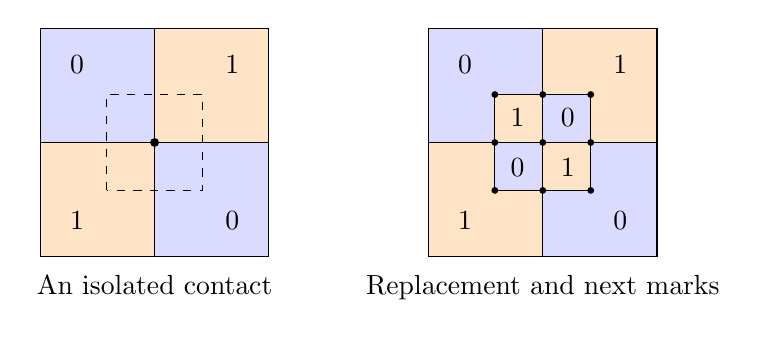
\begin{tikzpicture}[scale=1.45, line width=.45pt]
 \begin{scope}[xshift=-1.7cm]
  \fill[blue!14] (-1,0) rectangle (0,1);
  \fill[orange!22] (0,0) rectangle (1,1);
  \fill[blue!14] (0,-1) rectangle (1,0);
  \fill[orange!22] (-1,-1) rectangle (0,0);
  \draw (-1,-1) rectangle (1,1);
  \draw (-1,0)--(1,0) (0,-1)--(0,1);
  \draw[dashed] (-.42,-.42) rectangle (.42,.42);
  \node at (-.68,.68) {$0$}; \node at (.68,.68) {$1$};
  \node at (.68,-.68) {$0$}; \node at (-.68,-.68) {$1$};
  \fill (0,0) circle (1.1pt);
  \node[below] at (0,-1.08) {An isolated contact};
 \end{scope}
 \begin{scope}[xshift=1.7cm]
  \fill[blue!14] (-1,0) rectangle (0,1);
  \fill[orange!22] (0,0) rectangle (1,1);
  \fill[blue!14] (0,-1) rectangle (1,0);
  \fill[orange!22] (-1,-1) rectangle (0,0);
  \fill[orange!22] (-.42,0) rectangle (0,.42);
  \fill[blue!14] (0,0) rectangle (.42,.42);
  \fill[orange!22] (0,-.42) rectangle (.42,0);
  \fill[blue!14] (-.42,-.42) rectangle (0,0);
  \draw (-1,-1) rectangle (1,1);
  \draw (-1,0)--(1,0) (0,-1)--(0,1);
  \draw (-.42,-.42) rectangle (.42,.42);
  \node at (-.68,.68) {$0$}; \node at (.68,.68) {$1$};
  \node at (.68,-.68) {$0$}; \node at (-.68,-.68) {$1$};
  \node at (-.22,.22) {$1$}; \node at (.22,.22) {$0$};
  \node at (.22,-.22) {$1$}; \node at (-.22,-.22) {$0$};
  \foreach \x in {-.42,0,.42}
   \foreach \y in {-.42,0,.42}
    {\fill (\x,\y) circle (.85pt);}
  \node[below] at (0,-1.08) {Replacement and next marks};
 \end{scope}
\end{tikzpicture}
\caption{A four-sector example of the repair.  The square around the
contact is removed from every old tile, and its new sectors receive the
opposite labels.  Positive-length interfaces still join opposite labels.
Any same-label contacts involving the new tiles occur among the nine
marked points; the next, smaller removal separates them.  The proof also
allows any configuration of the eight permitted ray directions with
opposite labels in consecutive sectors.}
\label{geometry:repair-picture}
\end{figure}

We now verify that this procedure continues with uniform geometric
constants.  In particular, neither the separation constant nor the
isolation radius is allowed to deteriorate with the number of
generations.

\begin{lemma}[Uniform repair induction]
\label{geometry:repair-induction}
For a sufficiently small fixed choice of $a_0$ and the corresponding
threshold $S_*$, every active mark $(v,S)$ at every generation has a
terminal-square-free isolated star
$v+[-a_0S,a_0S]^2$ with the properties of
Lemma~\ref{geometry:initial-stars}.  Distinct active marks satisfy the same
separation inequality.  The simultaneous removal squares are disjoint.
Each replacement has opposite labels across every positive-length
interface of distinct identifiers, and its same-label contacts with old
remnants or peer replacements occur only at marks of the next generation.
Every descendant mark and every descendant birth region of a mark
$(v,S)$ lies within sup distance $2d(S)$ of $v$.  Each branch terminates
after finitely many generations.
\end{lemma}

\begin{proof}
Suppose the assertions hold at one generation.  By
\eqref{geometry:trim-margins}, the squares of radius $6d(S)$ are contained
in their parent stars.  They are also disjoint from all other current
removal squares.  Indeed for parent marks $(v,S),(w,T)$,
\[
 \norm{v-w}_\infty\ge a_0\max(S,T),\qquad
 6d(S)+d(T)\le \frac{7a_0}{1000}\max(S,T).
\]
Thus each modification sees only its parent's radial boundaries.

Across a new perimeter segment away from ray hits, the new interior
label was chosen opposite to the exterior label.  Across an interior
ray, the two labels remain opposite because the two exterior labels were
opposite.  All other positive-length interfaces are unchanged.  Contacts
not lying in the relative interior of one of these segments are among
the center, corners, or side midpoints of the new square.  This proves the
coloring and contact assertions.

Normalize one removal square to $[-1,1]^2$.  Its post-replacement
boundaries are subsets of the original eight radial rays together with
the four lines supporting this square.  The possible new marks are the
nine points of $\{-1,0,1\}^2$.  Every nonincident supporting line stays at
a fixed positive distance from a mark, and every other endpoint stays
at distance at least one.  Thus a fixed sufficiently small $a_0$ gives
an isolated radial star at each child, on the child's scale $d(S)$.
This is the same finite line configuration at every generation, so no
iteration of a shrinking constant is involved.

Two children of the same parent are at least $d(S)$ apart.  For children
of different parents their separation is at least
\[
 a_0\max(S,T)-d(S)-d(T)
 \ge \frac{a_0}{2}\max(S,T),
\]
which is larger than $a_0\max(d(S),d(T))$ by
\eqref{geometry:trim-margins}.  Their isolated-star squares therefore
satisfy the original separation invariant as well.

The child stars lie inside the parent star.  Consequently they avoid
all terminal squares from earlier generations.  A terminal square
created at another parent in the current generation is excluded by the
same cross-parent distance estimate.  For a direct statement covering
all later generations, each successive child displacement is at most
the preceding removal radius, and subsequent radii shrink by the fixed
factor at most $a_0/1000$.  Their sum, including the radius of the final descendant birth square,
is less than $2d(S)$.  Subtrees of distinct parents are therefore
separated by the preceding inequalities,
even if one subtree has already terminated.  This proves the asserted
terminal-square avoidance and descendant bound.

Finally, as long as a branch continues, its successive scales satisfy
$S_{j+1}=d(S_j)\le S_j^{\rho_0}$ with $\rho_0<1$.  After finitely many
steps the computed next halfside is below $S_*$, and that removal is
terminal.  This
completes the induction.
\end{proof}

All geometric edges avoid lattice sites.  Initially their vertices are
in $o+\Z^2$ because $r,s_k,t_k$ are dyadic integers, and the halfsizes and
midpoints used are integral.  In the recursion each new center, corner,
and midpoint is obtained by adding an integer vector to the preceding
center; the halfside $d(S)$ is an integer.  Enlarge $S_*$ once so that a
terminal halfside produced from $S\ge S_*$ is still at least two.
Every supporting line consequently has equation
\[
 x_1=o_1+m,\quad x_2=o_2+m,\quad
 x_1+x_2=o_1+o_2+m,\quad\text{or}\quad
 x_1-x_2=o_1-o_2+m,\qquad m\in\Z.
\]
None contains a point of $\Z^2$.  We may therefore use open actual tile
regions and closed birth regions without any convention for assigning a
lattice site on an interface.  The final open tile regions, the unaltered
part of the dummy region, and terminal-square interiors partition all
lattice sites.

\subsection{Separation from earlier actual regions}

Order tile identifiers as follows: all primaries first, all initial belt
tiles second, and then the replacement tiles by their generation of
birth.  Ties within each class can be broken arbitrarily.  The dummy tile
is excluded from this order.  Primaries already have the required
same-label separation from other primaries.  The next lemma handles all
remaining identifiers and explains why the order uses actual earlier
regions.

\begin{lemma}[Birth-template separation]
\label{geometry:birth-separation}
There is a fixed $c_1>0$ such that the following holds.  Let $\mathcal B$
be the closed birth region of an initial belt tile of side scale $u=t_k$,
or of a replacement tile whose removal square has halfside $u$.
Then its distance from the final actual region of every earlier or peer
identifier of the same label is at least $c_1u^{\rho_0}$.  A peer means
another initial belt tile, or another replacement born at the same
generation, respectively.
\end{lemma}

\begin{proof}
At the birth of an initial belt tile, compare its closure with the
primary and belt closures at that time.  At the birth of a replacement,
compare it with the old remnants \emph{after} that generation's removal
squares have been cut out, and with the peer replacements.  Each final
actual region is a subset of the corresponding compared region.  In
particular an ancestor is compared after its square has been removed;
its original birth region need not be disjoint from the new one.

Restrict attention to a closed box obtained by enlarging the tile's cell
or removal square by $2u$ in each direction.  Points outside this box are
at distance at least $2u$ from the birth region.  Translate by its cell
corner, or by its removal center, and rescale lengths by $u$.  Only
finitely many local pairs of closed regions can arise:
\begin{itemize}
\item
For belts, the nearby active lines and endpoints lie on the affine
quarter mesh, with their four prescribed slopes.  In a bounded box there
are only finitely many such lines and endpoints.  The local closures are
unions of faces of their arrangement; allowing all possible identifier
groupings still leaves only finitely many pairs of unions.  We classify
only the restrictions to this box: disconnected pieces of an identifier
outside it do not change the local pattern.
\item
For a replacement, the enlarged box lies in the isolated star of its
parent, by \eqref{geometry:trim-margins}.  It sees only the old radial
layout and the new square and sectors.  These lie on a fixed finite
arrangement in the rescaled coordinates.  Other parents' simultaneous
modifications do not enter this box.
\end{itemize}
Thus there is a common positive scale for the isolation neighborhoods
used in all these comparisons.

The two compared closures of the same label have no positive-length
interface.  Their intersections, if any, are contact marks by the belt
construction or Lemma~\ref{geometry:repair-induction}.  At a belt contact
the mark scale is comparable with $u$ (neighboring belt scales differ by
at most two); at a replacement contact it is $u$.  Choose disjoint open
contact squares of radius $\lambda u$ inside the isolated stars, for a
fixed sufficiently small $\lambda>0$.

First consider pairs of points $(x,y)$ in the two compared closures that
do not both belong to the same open contact square.  This condition
specifies a closed subset of the compact product of the two local
closures.  On it the distance $\norm{x-y}_\infty$ has a positive minimum:
if the minimum were zero, $x=y$ would be a common contact, and both points
would belong to its open contact square.  Since the list of rescaled
patterns is finite, the minimum is uniformly at least $c_2u$ whenever
this subset is nonempty.

It remains to consider $x,y$ in one contact star centered at $v$.
Inside that star each closure is a union of closed radial sectors.
Their direction sets are disjoint.  A shared direction would give a
shared ray segment, contrary to the absence of positive-length
same-label contacts.  Their boundary directions are among the eight
axis and diagonal directions, so the angle between their direction sets
is at least $\pi/4$.  Elementary Euclidean geometry, followed by
comparison of Euclidean and sup norms, gives
\begin{equation}
\label{geometry:angular-gap}
 \norm{x-y}_\infty
 \ge c_3\max\{\norm{x-v}_\infty,\norm{y-v}_\infty\}.
\end{equation}
For example, the squared Euclidean distance between radial vectors of
lengths $a,b$ and angle $\theta\ge\pi/4$ is
$(a-b)^2+2ab(1-\cos\theta)$, which bounds a fixed multiple of
$\max(a,b)^2$.

At the immediately following trim, the compared old or peer identifier
loses a square about $v$ of radius at least $c_4u^{\rho_0}$, by
\eqref{geometry:trim-radius} and comparability of mark scales.  This
removal also occurs if the square is terminal.  That identifier only
shrinks afterward.  Thus a point $y$ in its final actual region has
$\norm{y-v}_\infty\ge c_4u^{\rho_0}$, and
\eqref{geometry:angular-gap} supplies the required lower bound for pairs
inside the contact star.  Together with the preceding compactness
estimate and the exterior-of-box estimate this proves the lemma.
\end{proof}

The lemma compares the entire new birth region with an older actual
region.  Later deletions from the new tile are irrelevant to this
estimate.  This is the form needed for applying the collar estimate to
its untrimmed template and then discarding part of that template.

\subsection{Counting exceptional sites and verifying the templates}

Let an initial mark have scale $S$.  Along a branch,
$\log S_j\le\rho_0^j\log S$ until termination.  Its depth is therefore at
most
\[
 C+C\log\log(e^e+S).
\]
There are at most nine children per mark.  Consequently the number of
marks and replacements descended from this initial mark is at most
\begin{equation}
\label{geometry:descendant-count}
 C\bigl(\log(S+2)\bigr)^{C}.
\end{equation}
The constants are fixed; their magnitude is immaterial for a
size-independent area bound.  The scale of a mark initially belonging to
layer $k$ is comparable with $t_k$, and hence its logarithm is at most
$C(k+1)$.  By \eqref{geometry:belt-count}, the total number of belt tiles,
marks, and replacements is bounded by
\begin{equation}
\label{geometry:total-repairs}
 Cb\sum_{k\ge k_0}2^{-k\delta_0/2}(k+1)^C\le C'b.
\end{equation}
In particular this total is finite, even before restricting the
construction to the finite domain.

Each terminal square has halfside below the fixed $S_*$ and therefore
contains at most $C S_*^2$ lattice sites.  The dummy region has at most
$C|Z|$ cells of the fixed side $2^{k_0}$ and hence at most $Cb$ lattice
sites.  Let $D$ be the sites of $A$ that remain in the dummy identifier or
lie in terminal squares.  Sites overwritten by a replacement are no
longer counted as dummy sites.  Equations~\eqref{geometry:descendant-count}
and \eqref{geometry:total-repairs} give
\begin{equation}
\label{geometry:bad-sites}
 |D|\le Cb.
\end{equation}
This counts ambient sites and then intersects with $A$.  Missing sites,
holes, thin parts, and disconnected components of $\Lambda$ can only
reduce the count.

We now assign scanner scales to the birth templates.  Let
$T=\mathcal B\cap\Z^2$ for a birth region $\mathcal B$.
For a primary in layer $k$, take
\begin{equation}
\label{geometry:primary-scale}
 s_0=r=2^k,\qquad n=\left\lceil C_P r^{1+2\delta_0}\right\rceil.
\end{equation}
By \eqref{geometry:primary-pieces}, it has at most
$N_0\le C(s_k/r+2)^2\le C r^{2\delta_0}$ rectangular pieces, each of
sup-norm diameter at most $s_0$.  Choosing $C_P$ large ensures
\[
 n\ge C_{\mathrm{tpl}}N_0(s_0+1),\qquad
 \diam_\infty T\le s_k\le n.
\]
The birth template has endpoint distance at least $C_0r$, so the safe
clearance in Definition~\ref{scanner:template} follows from the choice
of $C_0$.  The exponent inequalities give, uniformly over primaries,
\begin{equation}
\label{geometry:primary-limits}
 L=\lfloor n^{1-\ell}\rfloor=o(r),\qquad
 n^\beta=o(t_k),\qquad n^\beta=o(r).
\end{equation}

For a belt tile take $u=t_k$, $s_0=u$, and
$n=\lceil C_Bu\rceil$.  It is a union of at most eight of the closed fan
triangles.  For a replacement whose removal halfside is $u$, take
$s_0=2u$ and $n=\lceil C_Bu\rceil$.  Subdivision into the triangles from
the center to corners and midpoints again uses at most eight pieces,
including for a wide sector or a homogeneous square.  Choose $C_B$ large
enough for all of these templates to satisfy
$n\ge C_{\mathrm{tpl}}N_0(s_0+1)$ and $\diam_\infty T\le n$.
In both cases $L=o(u)$.

Their cut clearance remains much larger than their size.  An initial
belt cell in $D_k$ has endpoint distance at least $C_0r$.
A mark on its closure has the same lower bound.  By
Lemma~\ref{geometry:repair-induction}, every descendant lies within
$2d(S)\le2t_k^{\rho_0}=o(t_k)$ of that mark.  After increasing $k_0$, all
its descendant birth templates therefore have endpoint distance at least
$(C_0-1)r$.  This also covers replacements extending into the dummy
region.  Since their side scales are at most $2t_k=o(r)$, their endpoint
distance exceeds both $4D_0s_0$ and $2n^\beta$.

These checks establish the exact geometric hypotheses of
Lemma~\ref{scanner:templates}.  In particular, for every birth template,
its dilated layers up to $L$ have the stipulated row and perimeter
bounds, and the safe-box estimate yields the core and shell entropy
bounds needed by Proposition~\ref{prop:collar}.  The verification uses
the finite union of convex pieces; no assertion that a primary, a sector
run, or its intersection with $A$ is a rectangle is needed.

For clarity, the relevant thresholds can be fixed in the following
order.  First fix $C_0,C_P,C_B$ and the absolute isolation constant.
Next increase $S_*$ until \eqref{geometry:trim-margins} holds, all belt and
replacement scanner scales are at least $n_*$, and
\begin{equation}
\label{geometry:fine-clearance}
 c_1u^{\rho_0}>2\lceil C_Bu\rceil^\beta
 \qquad(u\ge S_*).
\end{equation}
This is possible because $\rho_0>\beta$.  Finally increase $k_0$ to
ensure that initial belt scales exceed $S_*$, that all primary scales
exceed $n_*$, and that all the uniform large-scale inequalities just used
hold.  For primaries this includes their same-layer gap
$t_k>2n^\beta$, their nonadjacent-layer gaps, and
\eqref{geometry:primary-limits}.  Floors and ceilings only change fixed
multiplicative constants.

We can now finish the geometric proposition.  Retain just identifiers
whose final actual regions meet $A$, and let $X_i$ be those intersections,
ordered as above.  There are finitely many, since these nonempty sets
are pairwise disjoint subsets of a finite set.  They partition $A\setminus
D$, and each lies in its birth template.  Equations
\eqref{geometry:layer-distance}, \eqref{geometry:primary-limits}, and the
descendant clearance prove \eqref{geometry:cut-clearance}.
For primaries, earlier same-label primaries are separated by $t_k$ in the
same layer or by \eqref{geometry:nonadjacent} in other layers.  For belts
and replacements, Lemma~\ref{geometry:birth-separation} and
\eqref{geometry:fine-clearance} prove
\eqref{geometry:ordered-clearance}.  Restricting an older actual region
to $A$ preserves these lower bounds.

There are at most $Cb$ primaries per layer, and their scales satisfy
$n\ge c2^{(1+2\delta_0)k}$.  Their error sum is therefore bounded by
\[
 Cb\sum_{k\ge k_0}2^{-100(1+2\delta_0)k}\le C'b.
\]
The total number of other tiles is $O(b)$ by
\eqref{geometry:total-repairs}, and each has $n\ge1$.  Their error sum is
also $O(b)$.  This proves every assertion of
Proposition~\ref{prop:two-families}.

\subsection{Proof of the area law}

\begin{proof}[Proof of Theorem~\ref{thm:area}]
The empty domain and the empty or full region have zero entropy.
Put $b=|\partial_\Lambda A|$. If $b=0$,
Lemma~\ref{lem:zero-boundary} gives $S_\Omega(A)=0$.

Assume $b>0$.  Choose $n_*$ large enough for
Proposition~\ref{prop:collar} and Proposition~\ref{prop:amplification}
with $M=100$ to apply to the templates of
Proposition~\ref{prop:two-families}, uniformly with the stated template
bounds.  Increase it so that every radius $r$ supplied by amplification
at scale $n\ge n_*$ satisfies $L+2r<n^\beta$.  Let $D,X_i,T_i,n_i,f_i$ be the
resulting geometric decomposition, and put
\[
 S_i=A\cap\bigl(T_i+[-L_i,L_i]^2_{\Z}\bigr),\qquad
 J_i=(\Lambda\setminus A)\cup
       \bigcup_{\substack{j<i\\f_j=f_i}}X_j.
\]
Here $[-L_i,L_i]^2_{\Z}$ denotes the integer square.  For each $i$, let
$r_i$ be the radius supplied by amplification, using the size, boundary,
and information bounds from Proposition~\ref{prop:collar}.  The resulting
mutual-information estimate applies to $A\cap T_i$ against any sites
outside the graph neighborhood $N_{2r_i}^{\Lambda}(S_i)$.

We verify this condition for the whole set $J_i$, rather than for its
individual pieces.  A graph path of length at most $2r_i$ from $S_i$
stays within ambient distance $L_i+2r_i<n_i^\beta$ of $T_i$.
Equation~\eqref{geometry:ordered-clearance} excludes every earlier
same-family $X_j$ jointly.  Such a path also cannot reach
$\Lambda\setminus A$: its first crossing of the cut would put an endpoint
of a cut edge within that ambient distance of $T_i$, contradicting
\eqref{geometry:cut-clearance}.  Thus
\[
 J_i\subseteq\Lambda\setminus N_{2r_i}^{\Lambda}(S_i).
\]
Proposition~\ref{prop:amplification} and monotonicity under discarding
part of its first system yield
\[
 I_\Omega(X_i:J_i)
 \le I_\Omega(A\cap T_i:J_i)\le C n_i^{-100}.
\]
These estimates all concern the same original state $\Omega$, although
the auxiliary construction used to prove each estimate may differ.

Apply Lemma~\ref{geometry:cancellation} to the two labels.  Since each
site has dimension $q$,
\[
 S_\Omega(A)
 \le |D|\log q+\frac C2\sum_i n_i^{-100}
 \le C' b.
\]
Every choice of threshold and every constant in this proof depends only
on the fixed local dimension, interaction range and norm bound, and
spectral gap.  None depends on the size, shape, connectedness, or holes
of $\Lambda$, or on the choice of $A$.  This proves the theorem.
\end{proof}
